\section{简单的语音识别}
这个导航用来像你展示如何构建基本的语音识别网络识别不同的单词。对于了解真实的语音和识别更加复杂的系统是很重要的,但是像MNIST之于图像,它应该给你一个基本的技术方面的理解。当你完成这个导航后,你将有一个模型尝试分类一个音频段为‘yes‘,`no`,`up`,`down`,`left`,`right`,`on`,`of`,`stop`或者`go`。你将能在Andoird设备上运行它。
\subsection{准备}
你应该保证你已经安装了TensorFlow,因此脚本需要下载超过1GB的训练数据,你需要一个好的网络连接和有足够的存储空间的机器。训练过程可能花费几小时,确保你有一个机器长时间使用。
\subsection{Training}
开始训练处理,到Tensorflow源代码目录下运行:

\bashinline{python tensorflow/examples/speech_commands/train.py}
这个脚本开始下载\href{https://download.tensorflow.org/data/speech_commands_v0.01.tar.gz}{语音指令数据集},这个数据集包含65000人们说不同单词的音频波形文件。这个数据由Google手机基于CC BY许可释放,你可以通过\href{https://aiyprojects.withgoogle.com/open_speech_recording}{贡献5分钟你自己的声音}帮助改进数据集。压缩文件超过1GB,因此这部分也许会花点时间,但是你应该看到程序的日志,当它已经下载后你将不需要再次下载。

当下载完成后,你将看到像这样的采集数据:
\begin{bashcode}
I0730 16:53:44.766740   55030 train.py:176] Training from step: 1
I0730 16:53:47.289078   55030 train.py:217] Step #1: rate 0.001000, accuracy 7.0%, cross entropy 2.611571
\end{bashcode}
这显示了初始的处理和训练循环。你将看到每个训练步骤的训练输出信息。这里分隔意味着:
Step \#1显示我们的第一个训练步骤的循换开始。在这个例子中将总共有18000步,因此你可以查看到完成关闭的每一步。

rate 0.001000是训练的学习了率控制语音网络的权重更新。开始这个值是0.001,但是训练后期将减少10x到0.0001。

精度7.0\%是多少类别在训练中被正确的预测。预测的标签通过选择最高分的而选中。分数总是0-1之间,值越大代表对结果越有信心。

cross entropy 2.611571是损失函数的结果,这是通过比较当前训练和正确标签获得比较后的向量,这应该倾向于在训练中下载。在100步后,你应该看到类似这样的一行:
\begin{python}
|I0730 16:54:41.813438 55030 train.py:252] Saving to "/tmp/speech_commands_train/conv.ckpt-100"
\end{python}
这保存当前的训练权重到checkpoint文件。如果训练中断,你可以寻找最新的保存的checkpoint文件使用
\begin{python}
start_checkpoint=/tmp/speech_commands_train/conv.ckpt-100
\end{python}
命令行参数作为训练开始点。
\subsection{困惑矩阵}
在400步后,信息采集如下:
\begin{python}
I0730 16:57:38.073667   55030 train.py:243] Confusion Matrix:
 [[258   0   0   0   0   0   0   0   0   0   0   0]
 [  7   6  26  94   7  49   1  15  40   2   0  11]
 [ 10   1 107  80  13  22   0  13  10   1   0   4]
 [  1   3  16 163   6  48   0   5  10   1   0  17]
 [ 15   1  17 114  55  13   0   9  22   5   0   9]
 [  1   1   6  97   3  87   1  12  46   0   0  10]
 [  8   6  86  84  13  24   1   9   9   1   0   6]
 [  9   3  32 112   9  26   1  36  19   0   0   9]
 [  8   2  12  94   9  52   0   6  72   0   0   2]
 [ 16   1  39  74  29  42   0   6  37   9   0   3]
 [ 15   6  17  71  50  37   0   6  32   2   1   9]
 [ 11   1   6 151   5  42   0   8  16   0   0  20]]
\end{python}
第一部分为\href{https://www.tensorflow.org/api_docs/python/tf/confusion_matrix}{困惑矩阵}。为了明白它的意思,你首先需要知道正在使用的标签,在这个例子中为``silence``,``unknow``,``yes``,``no``,``up``,``down``,``left``,``right``,``on``,``off``,``stop``,``go``。每一列表示预测每个标签的样本,因此第一列表示所有的片段是``silence``,第二列表示为``unknow``,第三列为``yes``等等。

矩阵比单一分数更有用因为它给出了网络犯错的总结。在这个例子中你可以看到第一行所有的目录都为0,和初始的1隔开。因为第一行是所有的``silence``片段。这显示网络已经能从字中区别silence。

如果你看第一列,你看到一些非0值。这一列代表所有的片段被预测为silence,因此第一个cell正数是错误的。这意味真实话语中的一些片段实际上正在被用于预测slience,因此我们有一些错误正样本。

一个完美的模型将预测所有的词为0其它值在矩阵的中心。发现样例的区别可以找出模型如何更容易困惑,当你确定问题的时候你可以通过添加更多数据或者清理类别以确定问题。
\section{验证}
在困惑矩阵后,你应该看到这样一行:
\bash/I0730 16:57:38.073777 55030 train.py:245] Step 400: Validation accuracy = 26.3% (N=3093)/

一个好的实践是分开你的数据集为三类。最多的(在这个例子中大约80\%的数据)用于训练,小的数据集(10\%用于验证)用于评估训练中的精度,另一个集合(最后的10\%)用于评估训练完成后的精度。

分开的源映射网络将在训练中开始记忆它们的输入。通过设置分开验证,你将确保模型在从没见过的数据上工作。测试集保证你没有训练和验证集扭曲,不是一个输入的边界。

训练脚本自动分开数据集为三类,上面的采集行在验证集上显示模型的精度。最好是这应该接近训练精度。如果训练精度增加但是验证集没有,这是过拟合的信号,你的模型仅仅学习训练的片段没有生成广泛的泛化结果。
\subsection{TensorBoard}
一个好的可视化训练过程的方法是使用TensorBoard。默认,脚本保存输出时间到/tmp/retrain\_logs,你可以运行下面的代码载入\newline
\bashinline{tensorboard --logdir /tmp/retrain_logs}\newline
在你的浏览器中打开http://localhost:6006,你将看到node模型处理的表和图。
\begin{figure}[H]
\centering
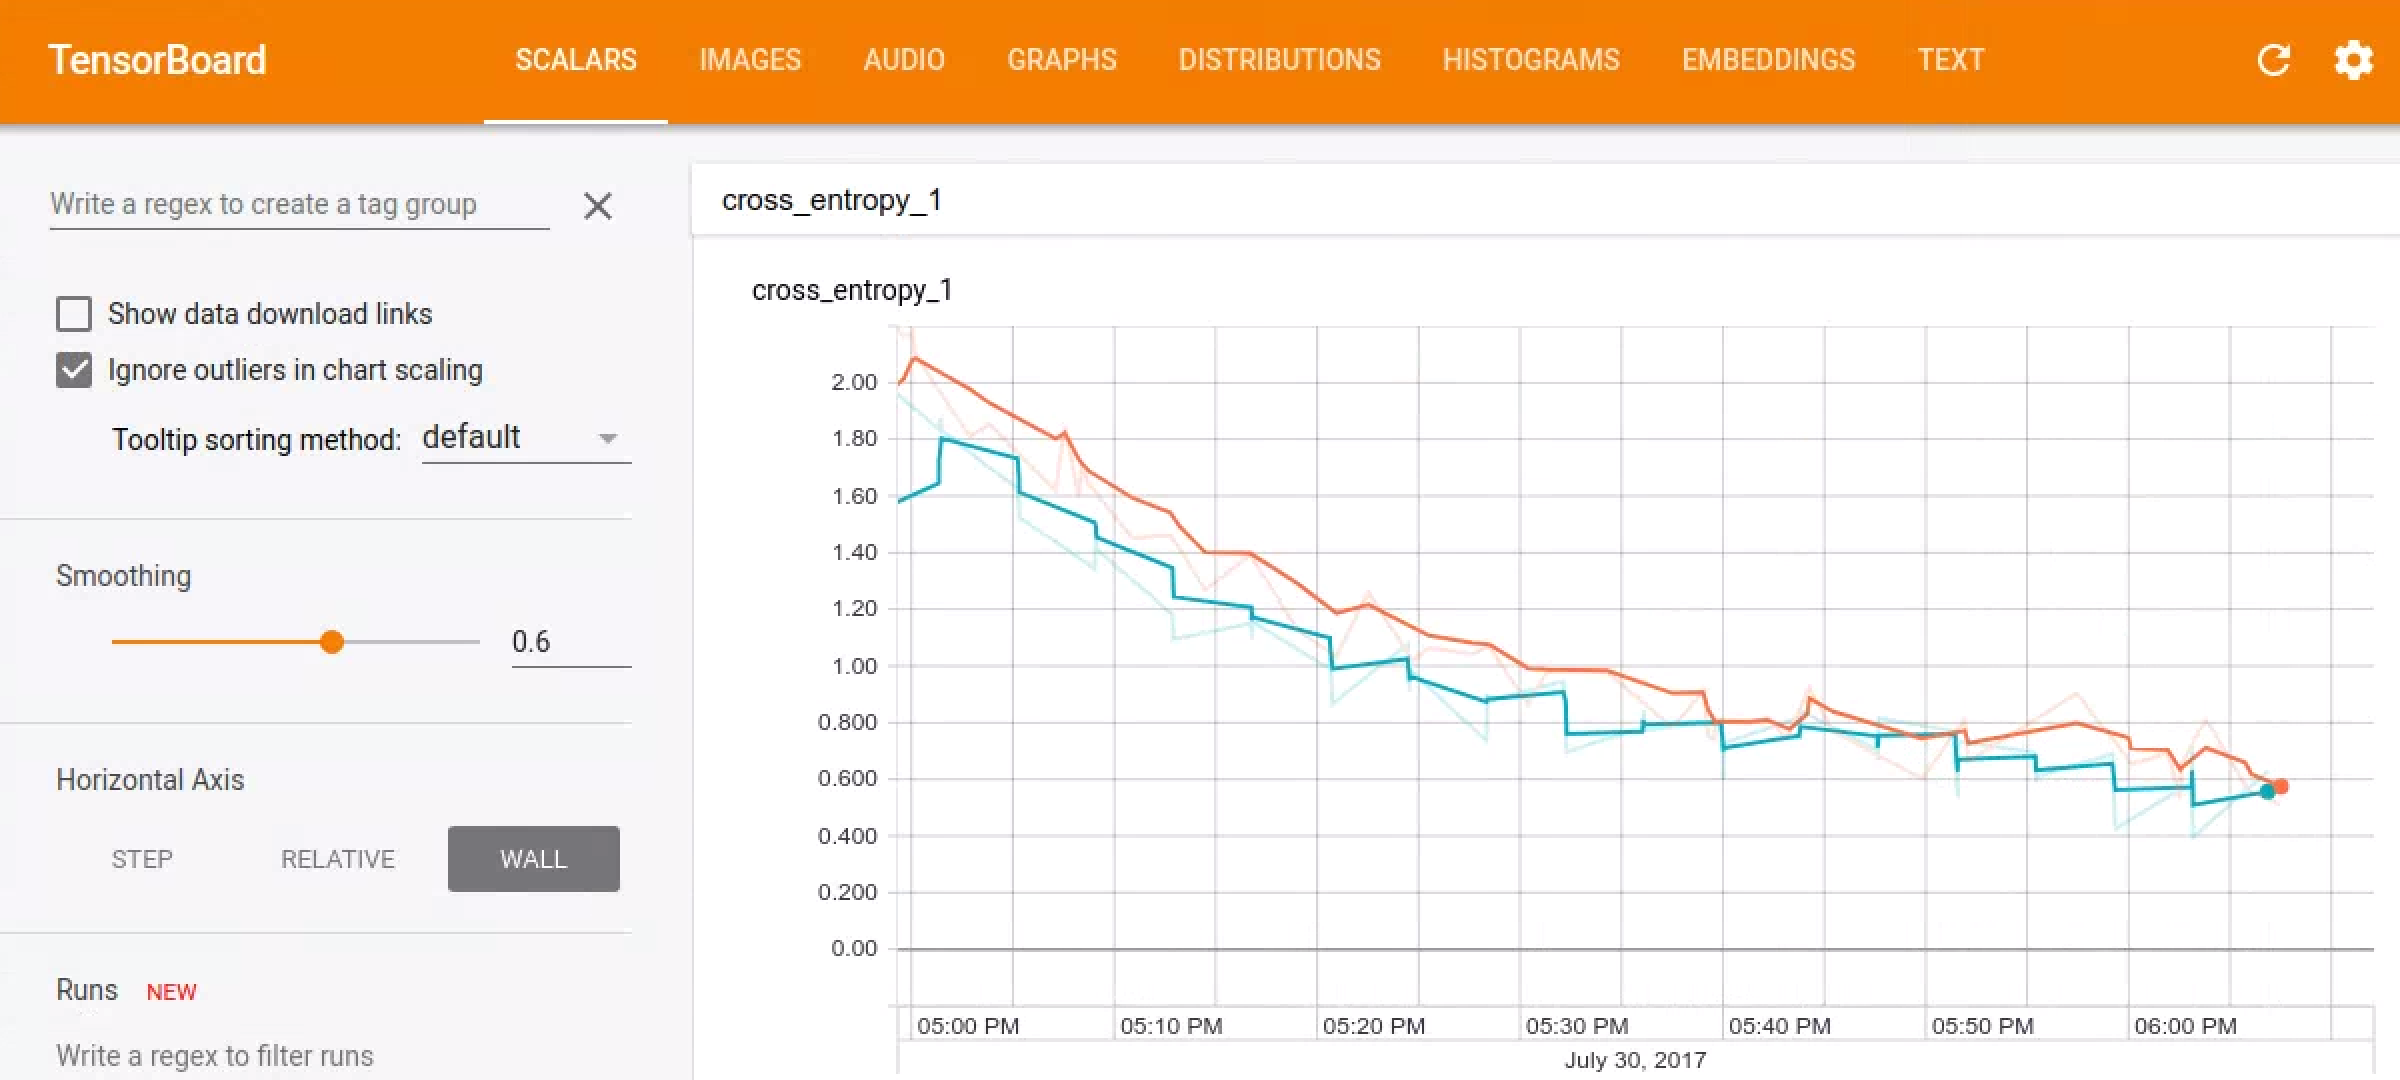
\includegraphics[scale=0.3]{speech_commands_tensorflow.png}
\caption{训练过程}
\end{figure}
\subsection{训练完成}
在集合小的训练后(依赖于你的机器的速度),脚本应该完成所有的18000步。它将打印出一个最后的困惑矩阵,沿着精度的得分,所有的测试集上的运行。结合默认设置,你应该看到精度在85\%到90\%之间。

因为语音识别对移动设备非常有用的,下一步我们将导出打包的格式在其它平台使用。为了做到这个,运行这个命令行:
\begin{bashcode}
python tensorflow/examples/speech_commands/freeze.py \
--start_checkpoint=/tmp/speech_commands_train/conv.ckpt-18000 \
--output_file=/tmp/my_frozen_graph.pb
\end{bashcode}
当冻结的模型被创建后,你将使用label\_wav.py脚本测试,像这样:
\begin{python}
python tensorflow/examples/speech_commands/label_wav.py \
--graph=/tmp/my_frozen_graph.pb \
--labels=/tmp/speech_commands_train/conv_labels.txt \
--wav=/tmp/speech_dataset/left/a5d485dc_nohash_0.wav 
\end{python}
这应该输出如下三个标签:
\begin{textcode}
left (score = 0.81477)
right (score = 0.14139)
_unknown_ (score = 0.03808)
\end{textcode}
有希望的``left``得分最高是正确的标签,因此训练是随机的,它也许不对应你尝试的第一个文件。得分在0和1之间,越高的值意味着模型对预测越有信心。
\subsection{在安卓app上运行模型}
简单的在真实应用中查看这个模型如何工作的方法是下载\href{https://github.com/tensorflow/tensorflow/tree/master/tensorflow/examples/android#prebuilt-components}{预编译的Android示例应用},安装它们在你的手机上,你将看到`TF Speech`出现在你的app列表中,打开它将显示一列在模型上训练的行为单词,用``Yes`开头或者``No``开头,当你给app权限使用microphone后,你应该能尝试说这些单词查看UI上识别的单词的高亮显示。

你也可以构建你自己的应用,因此打开\href{https://github.com/tensorflow/tensorflow/tree/master/tensorflow/examples/android#building-in-android-studio-using-the-tensorflow-aar-from-jcenter}{github仓库中可用的TensorFlow部分}。默认它下载\href{http://download.tensorflow.org/models/speech_commands_v0.01.zip}{默认一个tensorflow.org训练的模型},你可以使用\href{https://github.com/tensorflow/tensorflow/tree/master/tensorflow/examples/android#install-model-files-optional}{用你自己的模型取代它}。如果你这样做了,你将需要保证\href{https://github.com/tensorflow/tensorflow/tree/master/tensorflow/examples/android/src/org/tensorflow/demo/SpeechActivity.java}{主要的语音激活Java源文件}中的常数SAMPLE\_RATE和SAMPLE\_DURATION匹配任何你在训练中做的。你将看到有一个\href{https://github.com/tensorflow/tensorflow/tree/master/tensorflow/examples/android/src/org/tensorflow/demo/RecognizeCommands.java}{Java版本的识别命令模型},它和C++版本的很类似。如果你为它tweaked参数,你可以在SpeechActivity中更新它们在你的服务器测试中获得同样的结果。

示例app通过沿着你的冻结图根据标签text文件自动更新UI列表,这意味着你可以容易的尝试不同的模型改变代码。你将需要更新LABEL\_FILENAME和MODEL\_FILENAME如果你改变路径指定你添加的文件。

\subsection{这个模型如何工作}
这个导航的架构基于\href{http://www.isca-speech.org/archive/interspeech_2015/papers/i15_1478.pdf}{卷积神经网络用于小的封装的关键词发现}。它被选中因为它相对于顶尖的模型比较简单,训练快,容易理解。一些不同的方法结合音频构建神经网络模型,包括\href{https://svds.com/tensorflow-rnn-tutorial/}{训练神经网络}或者\href{https://deepmind.com/blog/wavenet-generative-model-raw-audio/}{dilated (atrous) convolutions}。这个导航基于卷积神经网络的类型对于处理过图像识别的人来说将很熟悉。这也许令人吃惊,尽管音频的内部是一个一维地连续信号,不是一个2维空间的问题。

我们通过定义时间窗解决这个问题,我们相信我们的说出的关键字将拟合进入,覆盖音频信号到图像中。这通过组合音频采样问题为短的片段,仅仅一些毫秒,计算带宽的频率强度/每个片段的频率强度被当做一个向量,这些向量被以时间排序形成二维数组。数组的值可以被当做单通的图像,被当做一个\href{https://en.wikipedia.org/wiki/Spectrogram}{spectrogram}。如果你想查看图像类别和音频采样输出,你可以运行`wav\_to\_spectrogram`工具。
\begin{bashcode}
bazel run tensorflow/examples/wav_to_spectrogram:wav_to_spectrogram -- \
--input_wav=/tmp/speech_dataset/happy/ab00c4b2_nohash_0.wav \
--output_png=/tmp/spectrogram.png 
\end{bashcode}
如果你打开/tmp/spectrogram.png你应看到下面:
\begin{figure}[H]
\centering
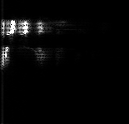
\includegraphics{spectrogram.png}
\caption{音频频谱}
\end{figure}
因为TensorFlow的内存顺序,在这个图像上的时间从顶部到底部增加,从左到右的频率进一步处理这个表达,返回它到一些\href{https://en.wikipedia.org/wiki/Mel-frequency\_cepstrum}{Mel-Frequency Cepstral Coefficients}或者简写为MFCC。这也有两个维度,一个通道表示因此它能被想图像一样处理。如果你目标是筒仓使得声音而不是你可与发现你可以跳过间隔直接操作频谱的语音。

图像的生成通过输入多层卷积神经网络,结合全连接和softmax。你可以在\href{https://github.com/tensorflow/tensorflow/tree/master/tensorflow/examples/speech_commands/models.py}{tensorflow/examples/speech\_commands/models.py}看到这个portion。
\subsection{流精度}
多数音频识别应用需要运行在连续的音频流上,而不是单个的片段。一个典型的方法是在这个环境中使用模型重复的在不同的时间偏移和在短的时间窗生成平滑预测。如果你将输入当做图像,它的连续的沿着时间轴滚动。我们想识别的单词可能在任何时刻,因此我们需要获取一系列快照改变对其捕获时间窗中的话语进入模型。如果我们采样率足够高,我们有机会在多个窗口捕获单词,因此平均结果提高了预测的可信度。

对于如何在流数据中使用我们的模型的例子,你可以查看\href{https://github.com/tensorflow/tensorflow/tree/master/tensorflow/examples/speech_commands/}{test\_streaming\_accuracy.c}。使用\href{https://github.com/tensorflow/tensorflow/tree/master/tensorflow/examples/speech_commands/recognize_commands.h}{RecognizeCommands}类运行通过一个长的输入音频,尝试发现单词,比较这些预测和标签列表。这使得应用在模型上的例子对于音频流是一个好的例子。

你需要一个长的音频文件测试它,沿着标签显示哪一个词被说了。如果你不想自己记录,你可以使用generate\_streaming\_test\_wave生成一些对称测试数据。通过将每个单词。这些单词来自你的当前数据集的测试,混合和背景噪声。为了运行它使用:\newline 
\bash|bazel run tensorflow/examples/speech_commands:generate_streaming_test_wav|
这将存储一个.wav文件到\text|/tmp/speech_commands_train/streaming_test.wav|添加一个文本列表标签到\text|/tmp/speech_commands_train/streaming_test_labels.txt|你可以运行测试:
\begin{bashcode}
bazel run tensorflow/examples/speech_commands:test_streaming_accuracy -- \
--graph=/tmp/my_frozen_graph.pb \
--labels=/tmp/speech_commands_train/conv_labels.txt \
--wav=/tmp/speech_commands_train/streaming_test.wav \
--ground_truth=/tmp/speech_commands_train/streaming_test_labels.txt \
--verbose
\end{bashcode}
这将输出关于正确匹配单词数量的信息和当没有真实世界说话时有多少次模型触发,有一些参数控制信号均衡工作,包含--average\_window\_ms设置时间长度到平均结果之上,--clip\_stride\_ms是模型应用间隔时间,--suppression\_ms停止从确定时间的子序列单词检测,--detection\_threshold控制固定结果前平均得分。

你想看到流精度输出三个数,而不是于在训练中的一个度量。这是因为不同的应用有不同的要求,一些能容忍在真实单词发现(高调用)中的频繁的错误结果,然而其它的每个注意力放在确保预测标签正确的可能性,即使没有检测(高精度)。一些工具给你一个你的模型如何在一个应用中执行的想法,你可以尝试tweak信号的平均参数调整给你你想要的性能。为了明白你的应用的正确的参数,你可以查看生成一个\href{https://en.wikipedia.org/wiki/Receiver_operating_characteristic}{RCOC curve}帮助你理解折中。
\subsection{识别命令}
流精度工具用一个简单的包含在C++类中的称为\href{https://github.com/tensorflow/tensorflow/tree/master/tensorflow/examples/speech_commands/recognize_commands.h}{RecognizeCommands}解码器。这个类被输入调整的TensorFlow模型的输出,它平滑信号,返回关于当你有足够信心考虑识别发现的单词。实现很小,仅仅记录一些预测和平均。因此容易按照需要port到其它的平台和语言。例如,方便的在安卓设备上做类似事情的Java level或者在树莓派上的Python。只要这些实现共享的同样的逻辑,你可以调整参数控制使用流测试工具的平滑,然后转化它们到你的程序中得到类似的结果。
\subsection{高级训练}
默认对于训练脚本在比较的小文件上产生好的端到端结果,但是有一些选项你可以改变来定制你自己要求的结果。
\subsection{常见的训练数据}
默认脚本将下载\href{https://download.tensorflow.org/data/speech_commands_v0.01.tgz}{语音命令数据集},但是你可以改变你的训练数据。为了在你自己的数据上训练,你应该确保你有至少100用于识别的录音,按照类别将它们放在文件夹中。例如,如果你尝试从猫的`miaow`识别狗叫`bark`,你将组织你的音频文件到合适的文件夹中。

为了指定脚本到你的新的音频文件,你将需要设置--adata\_url=禁用从语音命令数据集中下载,--data\_dir=/you/data/folder/找到你将创建的文件。为了文件本身应该是16位的little-endian PAM编码的WAVE格式。采样率波认为16000,但是只要所有你的音频是同样的采样率(脚本不支持重采样)米可以使用--sample\_rage参数改变它。片段应该有同样的长度。默认长度为1s,但是亦可以设置--clip\_duration\_ms flag。如果你有多个开头没有声音的片段,你可以找到单词对齐工具标准化它们(\href{https://petewarden.com/2017/07/17/a-quick-hack-to-align-single-word-audio-recordings/}{这里是一个方便直接的使用方法})

一个问题是查找出在你的数据集中同样声音的,如果你训练,验证,测试这可能误导衡量。例如,语音命令数据集有人重复相同的单词多次,每次表达可能和其它人很接近,因此,如果训练过拟合和memorizing one,它可能执行不可行当它看一个类似的在测试集中的复制是。为了避免这个危险,语音目录尝试确保所有的片段特征由单人说出的放在同一个部分中。片段基于文件名的hash值指定训练,测试或者验证集确保指定保留作为一个片段避免训练样本转移到其它的数据集。为了确保所有的给定的说话者的单词在同一个bucket,\href{https://github.com/tensorflow/tensorflow/tree/master/tensorflow/examples/speech_commands/input_data.py}{hash函数}当计算赋值的时候忽略文件名中在`nohash`之后的任何。这意味着如果你有像pets\_nohash\_o.wav和pete\_nohash\_1.wav的文件名,它们保证在同一个数据集。
\subsection{未知的类}
你的应用程序可能听到不在你的训练集中的程序,在这种情况下你将希望模型预测它不识别噪声。为了做这件事,你创建quack,oink和moo子文件夹用来自其它动物的噪声填充它们。--wanted\_words参数对于脚本定义你关心的类,所有的其它的注意在子文件夹中名字将用\_unknow\_类在训练的时候填充。语音目录数据集在未知的类中有20单词在unknow中,包含数字0-9和随机名称`Sheila`。

默认10\%训练样子被从未知类别中选中,但是你可以使用\textinline{unknown_percentage} 控制它。增加这将使得模型对于位置单词更少可能犯错,但是使得它太大可能适得其反正如模型可能决定它的最安全的分类所有的单词为未知。

\subsection{背景噪声}
真正的应用必须识别声音,即使是当有其它不相关的声音在环境中时也是。为了构建一个模型健壮的处理推理,我们需要结合类似特性训练录音。这文件在语音命令数据集中在多设备上通过在不同环境下的用户被捕获,没有在录音师,因此帮助添加真实性在训练中。为了添加更多,你可以在岁极端环境中混合音频到训练输入。在语音命令集中有一些特别的称为\_backgound\_noise\_的包含的一分钟长的带有白噪声和文件及其记录和每天的家庭活动波形文件的文件夹。

小的文件片段被随机选择用一个低的音量混在训练中混合。响度也随机选择,通过--background\_bolumn参数作为一个比例,这里0表示安静1表示音量最大。不是所有的片段都有片段添加在上面的,因此--background\_frequency标记控制混合的比例。

你的应用也许在它自己的环境中结合不同的背景噪声而不是这些默认的操作。因此你可以使用你的自己的音频段在\_backgound\_noise\_文件夹。这应该有相同的采样率作为你的主要的数据集,但是更长的周期以至于好的随机片段可以从它们当中选择。

\subsection{安静}
在多数情况下你关心的声音将断断续续,因此了解什么时候不匹配音频很重要。为了支持这点,有一个特殊的\_silence\_标签指明什么时候模型不感兴趣。因为在真实环境中没有完全的安静,我们实际上必须结合安静和相关的音频。为此我们重用\_background\_noise\_文件夹混合真实片段,通过--silence\_percentage放短的音频数据和feed这些在和真实数据用。正如位置的单词,设置更高可以权衡模型结果支持真正positive的安静,在错误负样本的代价,但是太大的一个比例可能是它掉进陷阱总是猜测处于安静状态。
\subsection{时间转换}
添加在背景噪声中是一个在用真实方法影响真实训练数据变形获取更多数据的方法,因此增加整体精度和时间偏移是另一个方法。这涉及时间上对训练样本数据的一个随机的偏移,因此一个小部分开始或者结束被减掉相反的部分被添加0。这在训练数据的开始mimics自然变量,通过--time\_shift\_ms标记控制,默认为100ms。添加值将提供更多的验证,但是风险是切断重要的音频部分。一个相关的是使用\href{https://en.wikipedia.org/wiki/Audio_time_stretching_and_pitch_scaling}{ time stretching and pitch scaling}参数扭曲,但是这超过了这个导航的范围。
\subsection{自定义模型}
默认用于这个脚本的模型很大,花费880亿FLOPS用于推理使用940000权重参数。在桌面机器上或者modern手机返回可用的语音,但是在设备交互速度受限资源涉及太多计算运行。为了支持这种情况有一对方法可以使用:
low\_latency\_conv基于cnn-on-stride4拓扑(描述在\href{http://www.isca-speech.org/archive/interspeech_2015/papers/i15_1478.pdf}{ Convolutional Neural Networks for Small-footprint Keyword Spotting paper}),精度比`conv`略微下降但是权重参数数量相同,每次运行预测需要1100万FLOPs,使得它变得更快。

为了使用这个模型,你将在命令行指定--model\_architecture=low\_lantency\_conv。你将需要更新训练率和每步数量,因此完整代码看起来如下:
\begin{bashcode}
python tensorflow/examples/speech_commands/train \
--model_architecture=low_latency_conv \
--how_many_training_steps=20000,6000 \
--learning_rate=0.01,0.001
\end{bashcode}
这要求脚本以0.001对2000步进行训练,然后使用10x更小的比率调整6000步。

low\_lantency\_svdf基于在\href{https://static.googleusercontent.com/media/research.google.com/en//pubs/archive/43813.pdf}{Compressing Deep Neural Networks using a Rank-Constrained Topology paper},精度将比`conv`小但是仅仅用7500000参数,更高效,这允许在测试的时候优化执行(例如当你实际上在你的应用中使用它),结果有750000FLOPs。

为了使用这个模型,你将在命令行指定--model\_architecture=low\_lantency\_svdf,更新训练比率和步数,因此完整的命令如下:
\begin{bashcode}
python tensorflow/examples/speech_commands/train \
--model_architecture=low_latency_svdf \
--how_many_training_steps=100000,35000 \
--learning_rate=0.01,0.005
\end{bashcode}
注意尽管比之前的两个拓扑要求更多的步骤,减少计算意味着训练应该花费相同时间,结果精度达到85\%。你可以在SVDF层改变这参数进一步调整拓扑计算和精度:
\begin{itemize}
	\item rank 近似排名(越高越好,但是结果是更多的计算。)
	\item num\_units 类似其它层类型,在层中指定节点数(越多节点,效果越好计算量越大)
\end{itemize}
忽略runtime,因此层允许通过缓存内部神经网络激活优化,你需要确保一个consistent stride(例如`clip\_stride\_ms`标记)然后冻结图,然后在流模型中执行模型(例如,test\_streaming\_accuracy.cc)。

其它参数的自定义,如果你想体验自定义模型,一个好的开始时tweak频谱图创造参数。这影响修改输入图像的大小,创建代码在\href{https://github.com/tensorflow/tensorflow/tree/master/tensorflow/examples/speech_commands/models.py}{models.py}中将调整计算数量和权重自动拟合不同的维度。如果你使得输入更小,模型将需要更小的计算处理它,因此它可以成为一个折中精度提高时延的方法。--window\_stride\_ms控制之前分析样本的频谱有多远。如果你增加这个值,给定时间内样本越少时间轴输入将缩小,--dct\_coefficient\_count标记控制多少bucket用于频率计数,因此减少这将其它维度缩减输入,--window\_size\_ms参数不影响大小,但是控制每个样本用于计算频谱的区域。减小输入训练样本的维度,你将需要确保所有的训练数据包含正确的初始片段部分。

如果在你的问题中你有一个完整的不同的模型,你也许可以plug它进入\href{https://github.com/tensorflow/tensorflow/tree/master/tensorflow/examples/speech_commands/models.py}{models.py}用余下的脚本处理预处理和训练机制。你将添加新的clause到create\_model,寻找你的架构的名字,然后调用模型创建函数。这函数给定频谱输入的大小对应的其它模型信息。希望创建TensorFlow操作读和处理输出预测向量,一个Placeholder控制dropout。余下的脚本处理整个模型为一个大图输入计算使用softmax和损失函数训练它。

一个常见的问题是当你调整模型训练超参数不是一个可以creep的值,多亏是数值精度问题。通常你可以通过减少像学习率和权重初始化函数,但是如果它们持续存在你可以使用--check\_nans标记追踪错误元。这将插入检测操作在TensorFlow操作中,当它们发生后训练将终止。

